\subsection{Hybrid}\label{Hybrid}

Hybrid processing is a mix of batch and real time \parencite{lewis2013content}.

Lets revisit roller coaster example. In batch scenario operator was waiting for 20 people to be seated. In hybrid scenario, we are expecting 20 people to show up. If there isn't enough people, operator will just start the ride with less than 20 people. One scenario would be business hours. In the morning and evening, we don't get as many people therefore operator is running the ride in hybrid mode but thought the noon (when there are core hours) operation seems like batch (but is hybrid on a grand scale).

Now lets consider our file ingestion from batch processing. We are still expecting n number of files. If we get n number of files, we start the processing with them (batch). Otherwise if we don't get all the files, we work with the files that were received as stream.

\begin{figure}[H]
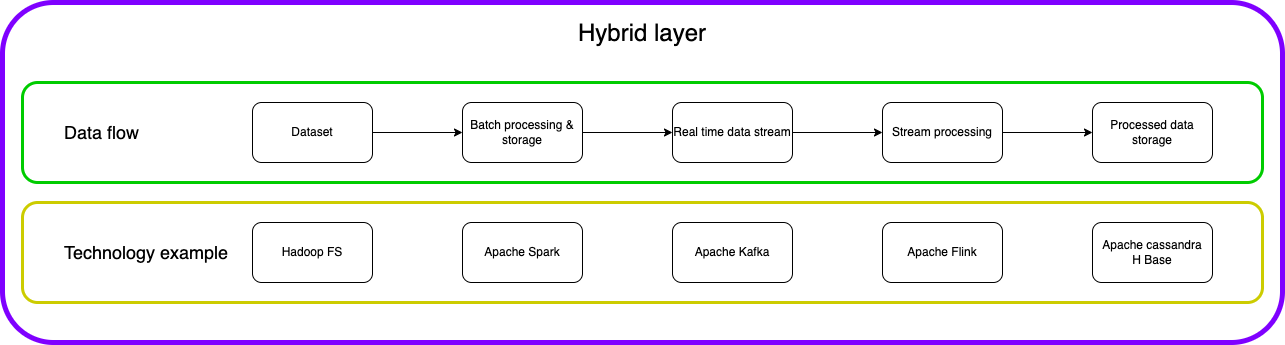
\includegraphics[scale=0.30]{img/ProcessingParadigms/BigData-HybridLayer.png}
\centering
\caption{Hybrid layer}
\label{fig:HybridLayer}
\end{figure}